\section{Digital Images}
\label{section:digital_image}
Digital images consist of discrete valued data points called pixels arranged in a grid where it is the value of these pixels that determine the appearance of the image. An image may be coloured, grayscale or binary depending on the format of the pixels that it's comprised of. A coloured pixel is represented by a three dimensional vector, Y, containing values for red, green and blue light.

\begin{equation}
  Y = \begin{bmatrix}
    R \\ G \\ B
  \end{bmatrix}
\end{equation}

The value range of the a coloured pixels elements R, G and B is set by the image's encoding, the JPEG format for example, has 8-bit encoding thus the value range for each element is $[0, 255]$ and so 16 million unique colours can be expressed. A grayscale image is comprised of single dimensioned pixels and is thus monochromatic being able to only represent the amount of light in an image but not its colour. A grayscale pixel's value is referred to as its \emph{intensity}. For an 8-bit encoded grayscale image its highest value is 255 and expresses white and its lowest value is 0 expressing black, in between these values are 254 shades of gray (see Figure \ref{fig:grayscale}). A binary image is represented by only black and white pixels whose values are either 0 or 1 respectively \cite{learnproc}. In image processing the format is selected based on the information that's important, in many situations only grayscale information is required because colour doesn't add any important information to the image. It is important to recognize which image format to use because computations are more expensive for a three dimensional coloured image than a single dimensioned grayscale or binary image. 

\begin{figure}[H]
  \centering
  \centering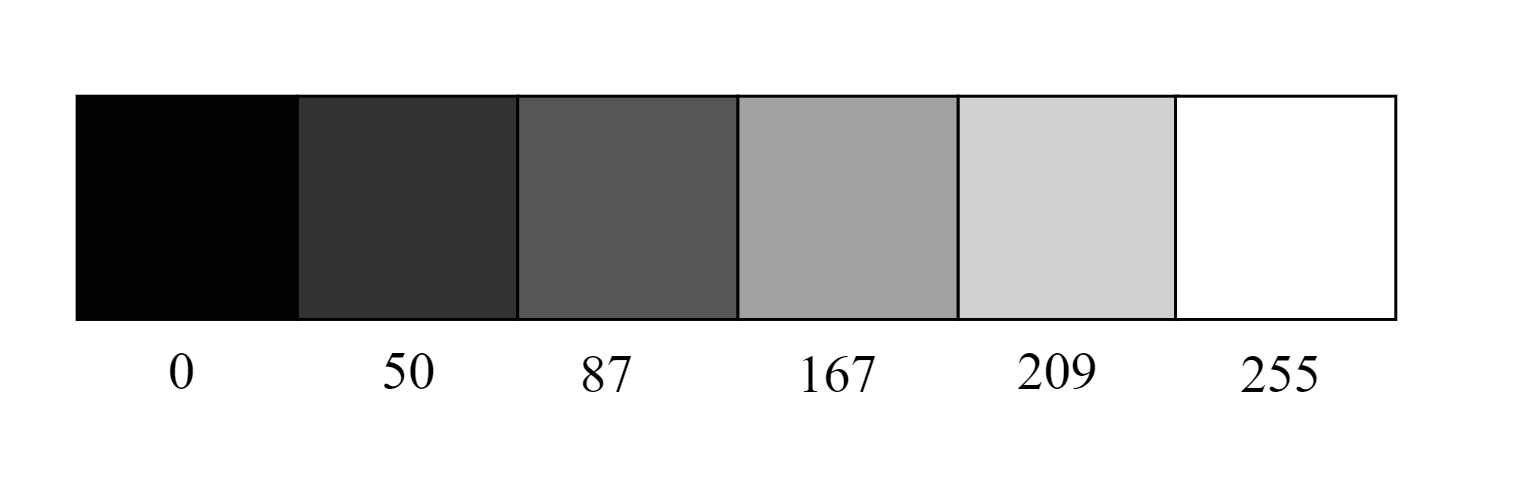
\includegraphics[width = 0.8\textwidth]{litreview/digital/grayscale}
  \caption{Grayscale value and colour range. Img: Learning Processing - Daniel Shiffman}
  \label{fig:grayscale}
\end{figure}

In software digital images are represented as an array of values where each cell corresponds to a pixel in the image and size of the array matches the resolution of the image. A colour image has a three dimensional array because it has two dimensions for resolution (image size) and another dimension for size of each pixels RGB vector, i.e. $M \times N \times 3$. Figure \ref{fig:2Darray} shows a simple grayscale image and its array representation.

\begin{figure}[H]
    \centering
    \begin{subfigure}[b]{0.5\linewidth}
      \centering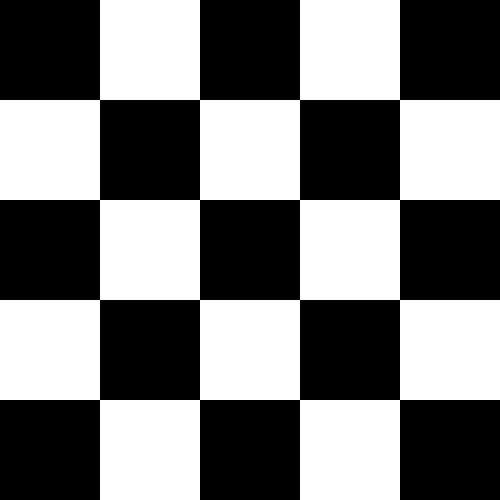
\includegraphics[width=150pt]{chessboard}
      \caption{\label{fig:fig1}}
    \end{subfigure}%
    \begin{subfigure}[b]{0.5\linewidth}
      \centering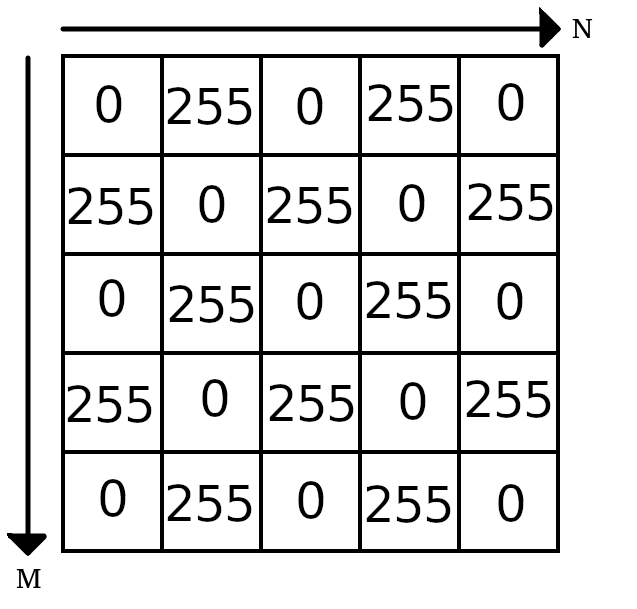
\includegraphics[width=150pt]{array2}
      \caption{\label{fig:fig2}}
    \end{subfigure}
    \caption{(\subref{fig:fig1}) A simple 8-bit grayscale image ~(\subref{fig:fig2}) Array representation of a grayscale image.}
    \label{fig:2Darray}
\end{figure}
  

The 2D array representation allows pixels to be referenced by their relative position in the $M$ and $N$ directions. Furthermore, $M$ and $N$ may be substituted for the x and y axes of the Cartesian plane. In fact, a digital image is just a sampled version of a two dimensional function where each pixel is described by a coordinate (x,y) and an intensity (z) at that point.

\begin{equation}
    z = f(x,y)
    \label{eq:2Dfunc}
\end{equation}

This representation is extremely useful as it means that two dimensional operations may be applied to a images. Rates of change, derivatives, of a digital images are important in computer vision because they help to identify features like lines and object edges. Figure \ref{fig:3Dplot} is a 3D plot of a 2D image where you can see that there is a rapid change in value between different coloured squares, shown as steep cliff edges. 

\begin{figure}[ht!]
  \centering
  \centering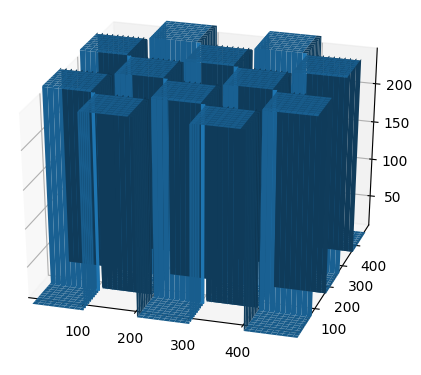
\includegraphics[width=150pt]{3Dchess}
  \caption{\label{fig:fig1} Surface Plot of Figure \ref{fig:2Darray}\ref{sub@fig:fig1}}
  \label{fig:3Dplot}
\end{figure}






